\documentclass[12pt,reqno]{amsart}

\usepackage{amsmath}
\usepackage{amsfonts}
\usepackage{graphicx}
%\usepackage{epstopdf}
\usepackage{hyperref}
\usepackage[left=1in,right=1in,top=0.9in,bottom=0.9in]{geometry}
\usepackage{multirow}
\usepackage{verbatim}
\usepackage{fancyhdr}
%\usepackage[small,compact]{titlesec} 

%\usepackage{pxfonts}
%\usepackage{isomath}
\usepackage{mathpazo}
%\usepackage{arev} %     (Arev/Vera Sans)
%\usepackage{eulervm} %_   (Euler Math)
%\usepackage{fixmath} %  (Computer Modern)
%\usepackage{hvmath} %_   (HV-Math/Helvetica)
%\usepackage{tmmath} %_   (TM-Math/Times)
%\usepackage{cmbright}
%\usepackage{ccfonts} \usepackage[T1]{fontenc}
%\usepackage[garamond]{mathdesign}
\usepackage{color}
\usepackage[normalem]{ulem}

\newtheorem{theorem}{Theorem}[section]
\newtheorem{conjecture}{Conjecture}[section]
\newtheorem{corollary}{Corollary}[section]
\newtheorem{lemma}{Lemma}[section]
\newtheorem{proposition}{Proposition}[section]
\theoremstyle{definition}
\newtheorem{assumption}{}[section]
%\renewcommand{\theassumption}{C\arabic{assumption}}
\newtheorem{definition}{Definition}[section]

\newtheorem{step}{Step}[section]
\newtheorem{remark}{Comment}[section]
\newtheorem{example}{Example}[section]
\newtheorem*{example*}{Example}

\linespread{1.1}

\pagestyle{fancy}
%\renewcommand{\sectionmark}[1]{\markright{#1}{}}
\fancyhead{}
\fancyfoot{} 
%\fancyhead[LE,LO]{\tiny{\thepage}}
\fancyhead[CE,CO]{\tiny{\rightmark}}
\fancyfoot[C]{\small{\thepage}}
\renewcommand{\headrulewidth}{0pt}
\renewcommand{\footrulewidth}{0pt}

\fancypagestyle{plain}{%
\fancyhf{} % clear all header and footer fields
\fancyfoot[C]{\small{\thepage}} % except the center
\renewcommand{\headrulewidth}{0pt}
\renewcommand{\footrulewidth}{0pt}}

\makeatletter
\renewcommand{\@maketitle}{
  \null 
  \begin{center}%
    \rule{\linewidth}{1pt} 
    {\Large \textbf{\textsc{\@title}}} \par
    {\normalsize \textsc{Paul Schrimpf}} \par
    {\normalsize \textsc{\@date}} \par
    {\small \textsc{University of British Columbia}} \par
    {\small \textsc{Economics 526}} \par
    \rule{\linewidth}{1pt} 
  \end{center}%
  \par \vskip 0.9em
}
\makeatother

\newcommand{\argmax}{\operatornamewithlimits{arg\,max}}
\newcommand{\argmin}{\operatornamewithlimits{arg\,min}}
\def\inprobLOW{\rightarrow_p}
\def\inprobHIGH{\,{\buildrel p \over \rightarrow}\,} 
\def\inprob{\,{\inprobHIGH}\,} 
\def\indist{\,{\buildrel d \over \rightarrow}\,} 
\def\F{\mathbb{F}}
\def\R{\mathbb{R}}
\newcommand{\gmatrix}[1]{\begin{pmatrix} {#1}_{11} & \cdots &
    {#1}_{1n} \\ \vdots & \ddots & \vdots \\ {#1}_{m1} & \cdots &
    {#1}_{mn} \end{pmatrix}}
\newcommand{\iprod}[2]{\left\langle {#1} , {#2} \right\rangle}
\newcommand{\norm}[1]{\left\Vert {#1} \right\Vert}
\newcommand{\abs}[1]{\left\vert {#1} \right\vert}
\renewcommand{\det}{\mathrm{det}}
\newcommand{\rank}{\mathrm{rank}}
\newcommand{\spn}{\mathrm{span}}
\newcommand{\row}{\mathrm{Row}}
\newcommand{\col}{\mathrm{Col}}
\renewcommand{\dim}{\mathrm{dim}}
\newcommand{\prefeq}{\succeq}
\newcommand{\pref}{\succ}
\newcommand{\seq}[1]{\{{#1}_n \}_{n=1}^\infty }
\renewcommand{\to}{{\rightarrow}}


\title{Differential Calculus}
\date{\today}

\begin{document}

\maketitle

%\section*{Midterm}

%\begin{itemize}
%\item Affine vs linear subspace (mistake I often make)
%\item Infinite unions and intersections
%\item 

In this lecture, we will define derivatives for functions on vector
spaces. We will show that all the familiar properties of derivatives
--- the mean value theorem, chain rule, etc --- hold in any vector
space. We will primarily focus on $\R^n$, but we also discuss infinite
dimensional spaces (will we need to differentiate in them to study
optimal control later). All of this material is also covered in
chapter 4 of Carter. Chapter 14 of Simon and Blume and chapter 9 of
Rudin's \textsl{Principles of Mathematical Analysis} cover
differentiation on $\R^n$. Simon and Blume is better for general
understanding and applications, but Rudin is better for proofs and
rigor. 

\section{Derivatives}

\subsection{Partial derivatives}
We have discussed limits of sequences, but perhaps not limits of
functions. To be complete, we define limits as follows.
\begin{definition}
  Let $X$ and $Y$ be metric spaces and $f:X \to Y$.
  \[ \lim_{x \to x_0} f(x) = c \]
  where $x$ and $x_0 \in X$ and $c \in Y$, 
  means that $\forall \epsilon > 0$ $\exists \delta > 0$ such that
  $d(x,x_0) < \delta $ implies $d(f(x),c) < \epsilon$. 
\end{definition}
Equivalently, we could say $ \lim_{x \to x_0} f(x) = c $ means that
for any sequence $\{x_n\}$ with $x_n \to x$, $f(x_n) \to c$. 

You are probably already familiar with the derivative of a function of
one variable. Let $f: \R \to \R$. $f$ is differentiable at $x_0$ if 
\[ \lim_{h \to 0} \frac{f(x_0 + h) - f(x_0)}{h} = \frac{d
  f}{dx}(x_0) \]
exists. Similiarly, if $f: \R^n \to \R$ we define its $i$th partial
derivative as follows.
\begin{definition}
  Let $f:\R^n \to R$. The $i$th \textbf{partial derivative} of $f$ is 
  \[ \frac{\partial f}{\partial x_i} (x_0) = \lim_{h \to 0}
  \frac{f(x_{01},...,x_{0i}, ... x_{0n})}{h}. \]
\end{definition}
The $i$th partial derivative tells you how much the function changes
as its $i$th argument changes.
\begin{example}
  Let $f:\R^n \to \R$ be a production function. Then we call
  $\frac{\partial f}{\partial x_i}$ the \textbf{marginal product} of
  $x_i$. If $f$ is Cobb-Douglas, $f(k,l) = Ak^\alpha l^\beta$, where
  $k$ is capital and $l$ is labor, then the marginal products of
  capital and labor are
  \begin{align*}
    \frac{\partial f}{\partial k} (k,l) = & A \alpha k^{\alpha-1}
    l^\beta \\
    \frac{\partial f}{\partial l} (k,l) = & A \beta k^{\alpha}
    l^{\beta -1}.
  \end{align*}
\end{example}

\subsection{Examples}
\begin{example}
  If $u:\R^n \to \R$ is a utility function, then we call
  $\frac{\partial u}{\partial x_i}$ the marginal utility of $x_i$.  
  If $u$ is CRRA, 
  \[u(c_1,...,c_T) =
  \sum_{t=1}^T \beta^t \frac{c_t^{1-\gamma}}{1-\gamma} \]
  then  the marginal utility of consumption in period $t$ is 
  \[ \frac{\partial u}{\partial c_t} = \beta^t c_t^{-\gamma}. \]
\end{example}

\begin{example}
  The price elasticity of demand is the percentage change in demand
  divided by the percentage change in its price. If $q_1:\R^3 \to \R$ is
  a demand function with three arguments: own price $p_1$, the price
  of another good, $p_2$, and consumer income, $y$.  The own price
  elasticity is 
  \[ \epsilon_{q_1,p_1} = \frac{\partial q_1}{\partial p_1}
  \frac{p_1}{q_1(p_1,p_2,y)}. \]
  The cross price elasticity is the percentage change in demand
  divided by the percentage change in the other good's price, i.e.
  \[ \epsilon_{q_1,p_2} = \frac{\partial q_1}{\partial p_2}
  \frac{p_2}{q_1(p_1,p_2,y)}. \]
  Similarly, the income elasticity of demand is
  \[ \epsilon_{q_1,y} = \frac{\partial q_1}{\partial y}
  \frac{y}{q_1(p_1,p_2,y)}. \]
\end{example}

\subsection{Total derivatives}

Derivatives of univariate functions have a number of useful properties
that partial derivatives do not always share. Examples of useful
properties include univariate derivatives giving the slope of a
tangent line, the implicit function theorem, and Taylor series
approximations. We would like the derivatives of multivariate
functions to have these properties, but partial derivatives are not
enough for this.

\begin{example}\label{ex:nondiff}
  Consider $f:\R^2 \to \R$, 
  \[ f(x,y) = \begin{cases} x^2+y^2 & \text{ if } xy < 0 \\
    x + y \text{ if } xy \geq 0 
  \end{cases}
  \]
  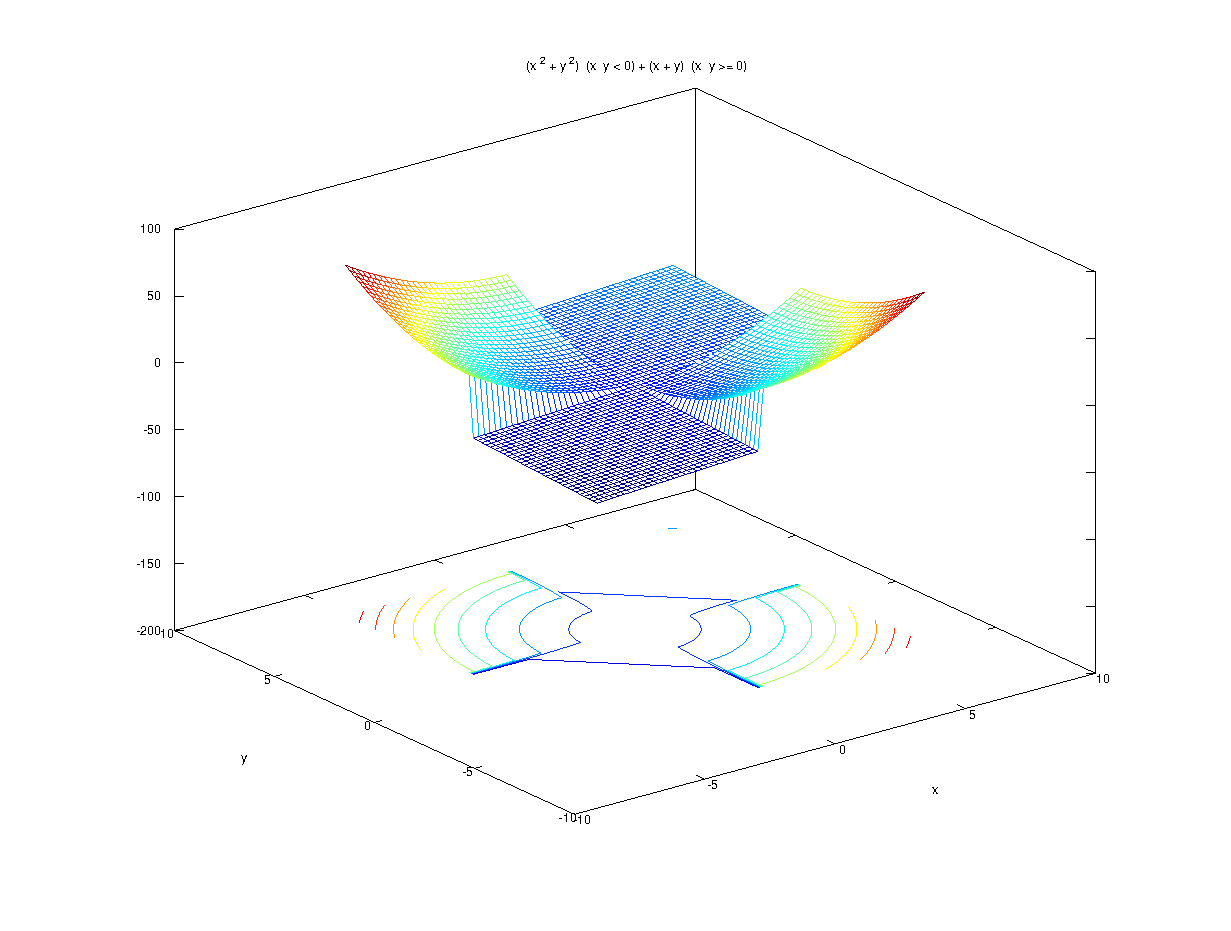
\includegraphics[width=\linewidth]{nondiff}
  
  The partial derivatives of this function at $0$ are $\frac{\partial
    f}{\partial x}(0,0) = 1$ and $\frac{\partial f}{\partial y}(0,0) =
  1$. However, there are points arbitrarily close to zero with
  $\frac{\partial f}{\partial x}(x,y) = 2x + 2y$. If we were to try to
  draw a tangent plane to the function at zero, we would find that we
  cannot. Although the partial derivatives of this function exist
  everywhere, it is in some sense not differentialable at zero (or
  anywhere with $xy = 0$).
\end{example}
Partially motivated by the preceding example, we define the
total derivative (or just the derivative; we're saying ``total'' to
emphasize the difference between partial derivatives and the derivative).
\begin{definition}
  Let $f: \R^n \to \R$. The \textbf{derivative} (or total derivative
  or differential) of $f$ at $x_0$ is a  linear mapping, $Df_{x_0}:
  \R^n \to \R^1$ such that
  \begin{align*}
    \lim_{h \to 0} \frac{\left|f(x_0 + h) - f(x_0) - Df_{x_0} h\right|} {\norm{h}}
    = 0.
  \end{align*}
\end{definition}
The $h$ in this definition is an $n$ vector in $\R^n$. This is
contrast to the $h$ in the definition of partial derivatives, which
was just a scalar. The fact that $h$ is now a vector is important
because $h$ can approach $0$ along any path. Partial derivatives only
look at the limits as $h$ approaches $0$ along the axes. This allows
partial derivatives to exist for strange functions like the one in
example \ref{ex:nondiff}. We can see that the function from the
example is not differentiable by letting $h$ approach $0$ along a path
that switches from $xy<0$ to $xy\geq 0$ infinitely many times close to
$0$. The limit in the definition of the derivative does not exist
along such a path, so the derivative does not exist. 
\begin{remark}
  In proofs, it will be useful to define $r(x,h) = f(x+h) - f(x) -
  Df_x h$. We will then repeatedly use the fact that $\lim_{h \to 0}
  \frac{|r(x,h)|}{\norm{h}} = 0$.
\end{remark}

If the derivative of $f$ at $x_0$ exists, then so do the partial
derivatives, and the total derivative is simply the $1 \times n$
matrix of partial derivatives.
\begin{theorem}\label{thm:tdiff}
  Let $f: \R^n \to \R$ be differentiable at $x_0$, then
  $\frac{\partial f}{\partial x_i}(x_0)$ exists for each $i$ and 
  \[ Df_{x_0} h = \begin{pmatrix} \frac{ \partial f}{\partial x_1}(x_0) &
    \cdots \frac{ \partial f}{\partial x_n }(x_0)
  \end{pmatrix} h. \]
\end{theorem}
\begin{proof}
  Since $f$ is differentiable at $x_0$, we can make $h = e_i t$ for
  $e_i$ the $i$th standard basis vector, and $t$ a scalar. The
  definition of derivative says that
  \begin{align*}
    \lim_{t \to 0} \frac{\left|f(x_0 + e_i t) - f(x_0) - Df_{x_0} (e_i t)\right|}
    {\norm{e_i t} } & = 0.
  \end{align*}
  Let 
  \begin{align*}
    r_i(x_0,t) = f(x_0 + e_i t) - f(x_0) - t D f_{x_0} e_i 
  \end{align*}
  and note that $\lim_{t \to 0} \frac{|r_i(x_0,t)|}{|t|} =
  0$. Rearranging and dividing by $t$, 
  \begin{align*}
    \frac{f(x_0 + e_i t) - f(x_0)}{t} = D f_{x_0} e_i + \frac{r_i(x_0,t)}{t}
  \end{align*}
  and taking the limit
  \begin{align*}
    \lim_{t \to 0} \frac{f(x_0 + e_i t) - f(x_0)}{t} = D f_{x_0} e_i 
  \end{align*}
  we get the exact same expression as in the definition of the partial
  derivative. Therefore, $\frac{\partial f}{\partial x_i} = D
  f_{x_0}e_i$. Finally, as when we first introduced matrices, we know
  that linear transformation $D f_{x_0}$ must be represented by
  \[ Df_{x_0} h = \begin{pmatrix} \frac{ \partial f}{\partial x_1}(x_0) &
    \cdots \frac{ \partial f}{\partial x_n }(x_0)
  \end{pmatrix} h. \]
\end{proof}
We know from example \ref{ex:nondiff} that the converse of this
theorem is false. The existence of partial derivatives is not enough
for a function to be differentiable. However, if the partial
derivatives exist and are continuous in a neighborhood, then the
function is differentiable. 
\begin{theorem}\label{thm:ptdiff}
  Let $f:\R^n \to \R$ and suppose its partial derivatives exist and
  are continuous in $N_\delta(x_0)$ for some $\delta>0$. Then $f$
  is differentiable at $x_0$ with 
  \[ Df_{x_0}= \begin{pmatrix} \frac{ \partial f}{\partial x_1}(x_0) &
    \cdots \frac{ \partial f}{\partial x_n }(x_0)
  \end{pmatrix}. \]
\end{theorem}
\begin{proof}
  Let $h = (h_1, ..., h_n)$ with $\norm{h}<r$. Notice that
  \begin{align} 
    f(x_0+h) - f(x_0) = & f(x_0 + h_1 e_1) - f(x_0) + f(x_0+h_1 e_1 +
    h_2 e_2) - f(x_0 + h_1 e_1) + ... \\
    & + f(x_0 + h) - f\left(x_0 -
    \sum_{i=1}^{n-1} h_i e_i\right) \\
    &  = \sum_{j=1}^n f\left(x_0 + \sum_{i=1}^j h_i e_i\right) -
    f\left(x_0 + \sum_{i=1}^{j-1} h_i e_i\right). \label{eq:earlier}
  \end{align}
  By the mean value theorem (\ref{thm:mvt}), 
  \[ f\left(x_0 + \sum_{i=1}^j h_i e_i\right) -
  f\left(x_0 + \sum_{i=1}^{j-1} h_i e_i\right) = h_j \frac{\partial f}
  {\partial x_j} (x_0 +  \sum_{i=1}^{j-1} h_i e_i + \bar{h}_je_j) \]
  for some $\bar{h}_j$ between $0$ and $h_j$.  The partial derivatives
  are continuous by assumption, so by making $r$ small enough, we can
  make  
  \[\left| \frac{\partial f}
    {\partial x_j} (x_0 +  \sum_{i=1}^{j-1} h_i e_i + \bar{h}_je_j) -
    \frac{\partial f}{\partial x_j}(x_0) \right| < \epsilon /n, \]
  for any $\epsilon>0$. 
  Combined with equation \ref{eq:earlier} now we have,
  \begin{align} 
    f(x_0+h) - f(x_0) = & \sum_{j=1}^n  h_j \left(\frac{\partial f}{\partial
        x_j} (x_0) + \frac{\epsilon}{n}\right) \\
    \left| f(x_0+h) - f(x_0)  - \sum_{j=1}^n  h_j \frac{\partial f}{\partial
        x_j} (x_0) \right| = & \left| \sum_{j=1}^n h_j \epsilon/n \right|
    \\
    \left| f(x_0+h) - f(x_0)  - Df_{x_0} h \right| \leq & \epsilon
    \norm{h} 
  \end{align}
  Dividing by $\norm{h}$ and taking the limit, 
  \[ \lim_{h \to 0} \frac{\left| f(x_0+h) - f(x_0)  - Df_{x_0} h
    \right|}{\norm{h}} \leq \epsilon.
  \]
  This is true for any $\epsilon>0$, so the limit must be 0. 
\end{proof}
A minor modification of this proof would show the stronger result that
$f:\R^n \to \R$ has a continuous derivative on an open set $U
\subseteq \R^n$ if and only if its partial derivatives are continuous
on $U$. We call such a function \textbf{continuously differentiably}
on $U$ and denote the set of all such function as $C^1(U)$. 

\subsection{Mean value theorem}

The mean value theorem in $\R^1$ says that $f(x+h) - f(x) =
f'(\bar{x}) h$ for some $\bar{x}$ between $x+h$ and $x$. The same
theorem holds for multivariate functions. To prove it, we will need a
couple of intermediate results. Recall the following from the midterm
review. 
\begin{theorem}
  Let $f:\R^n \to \R$ be continuous and $K \subset \R^n$ be
  compact. Then $\exists x^* \in K$ such that $f(x^*) \geq f(x)
  \forall x \in K$. 
\end{theorem}
Simon and Blume call this Weierstrass's theorem (30.1). 
\begin{definition}
  Let $f: \R^n \to \R$. we say that $f$ has a local maximum at $x$ if
  $\exists \delta > 0$ such that $f(y) \leq f(x)$ for all $y \in
  N_\delta(x)$. 
\end{definition}
Next, we need a result that relates derivatives to maxima. 
\begin{theorem}
  Let $f: \R^n \to \R$ and suppose $f$ has a local maximum at $x$ and
  is differentiable at $x$. Then $Df_x = 0$. 
\end{theorem}
\begin{proof}
  Choose $\delta$ as in the definition of a local maximum. Since $f$
  is differentiable, we can write
  \[ \frac{f(x+h) - f(x)}{\norm{h}} =\frac{ Df_x h +
    r(x,h)}{\norm{h}} \] where $\lim_{h \to 0}
  \frac{|r(x,h)|}{\norm{h}} = 0$. Let $h = t v$ for some $v \in \R^n$
  with $\norm{v} =1$ and $t \in \R$. If $D f_x v > 0$, then for $t>0$
  small enough, we would have $\frac{f(x+tv) - f(x)}{|t|} = D
  f_x v + \frac{r(x,tv)}{|t|} > D
  f_x v / 2 > 0$ and $f(x+tv)> f(x)$ in contradiction to $x$ being a
  local maximum. Similary, if $D f_v v < 0$ then for $t<0$ and small,
  we would have $\frac{f(x+tv) - f(x)}{|t|} = D
  -f_x v + \frac{r(x,tv)}{|t|} > -D
  f_x v / 2 > 0$ and $f(x+tv)> f(x)$. Thus, it must be that $D f_x v =
  0$ for all $v$, i.e. $D f_x = 0$. 
\end{proof}
Now we can prove the mean value theorem.
\begin{theorem}[mean value]\label{thm:mvt}
  Let $f:\R^n \to \R^1$ be in $C^1(U)$ for some open $U$. Let $x, y
  \in U$ be such that the line connecting $x$ and $y$, $\ell(x,y) =
  \{z\in \R^n: z = \lambda x + (1-\lambda) y, \lambda \in [0,1]\}$, is
  also in $U$. Then there is some $\bar{x} \in \ell(x,y)$ such that
  \[ f(x) - f(y) = Df_{\bar{x}} (x-y). \]
\end{theorem}
\begin{proof}
  Let $z(t) = y + t(x-y)$ for $t \in [0,1]$ (i.e.
  $t=-(1-\lambda)$). Define
  \[ g(t) = f(y) - f(z(t)) + \left(f(x) - f(y)\right) t \] Note that
  $g(0) = g(1) = 0$. The set $[0,1]$ is closed and bounded, so it is
  compact. It is easy to verify that $g(t)$ is continuously
  differentiable since $f$ is continuously differentiable . Hence, $g$
  must attain its maximum on $[0,1]$, say at $\bar{t}$. If $\bar{t} =
  0$ or $1$, then either $g$ is constant, in which case $f$ is
  constant and $Df = 0$, so the theorem is true, or $g$ must have an
  interior minimum, and we can look at the maximum of $-g$
  instead. When $\bar{t}$ is not $0$ or $1$, then the previous theorem
  shows that $g'(\bar{t}) = 0$. Simple calculation shows that
  \[ g'(\bar{t}) = -Df_{z(\bar{t})} (x-y) +  f(x) - f(y) = 0 \]
  so 
  \[ Df_{\bar{x}}(x-y) = f(x) - f(y) \]
  where $\bar{x} = z(\bar{t})$.
\end{proof}

\subsection{Functions from $\R^n \to \R^m$}

So far we have only looked at functions from $\R^n$ to $\R$. Functions
to $\R^m$ work essentially the +same way. 
\begin{definition}
  Let $f: \R^n \to \R^m$. The \textbf{derivative} (or total derivative
  or differential) of $f$ at $x_0$ is a linear mapping, $Df_{x_0}:
  \R^n \to \R^m$ such that
  \begin{align*}
    \lim_{h \to 0} \frac{\left\Vert f(x_0 + h) - f(x_0) - Df_{x_0}
        h\right\Vert} {\norm{h}} = 0. 
  \end{align*}
\end{definition}
Theorems \ref{thm:tdiff} and \ref{thm:ptdiff} sill hold with no
modification. The total derivative of $f$ can be represented by the
$m$ by $n$ matrix of partial derivatives,
\[ Df_{x_0}  = \begin{pmatrix} \frac{\partial f_1}{\partial x_1}(x_0) &
  \cdots & \frac{\partial f_1}{\partial x_n}(x_0) \\
  \vdots & & \vdots \\
  \frac{\partial f_m}{\partial x_1}(x_0) & \cdots & \frac{\partial
    f_m}{\partial x_n}(x_0)  
\end{pmatrix}. \] 
This matrix of partial derivatives is often called
the \textbf{Jacobian} of $f$. 

The mean value theorem \ref{thm:mvt} holds for each of the component
functions of $f:\R^n \to \R^m$. Meaning, that $f$ can be written as
$f(x) = \begin{pmatrix} f_1(x) & \cdots & f_m(x) \end{pmatrix}^T$
where each $f_j:\R^n \to \R$. The mean value theorem is true for each
$f_j$, but the $\bar{x}$'s will typically differ with $j$.
\begin{corollary}[mean value for $\R^n \to \R^m$]\label{thm:mvtm}
  Let $f:\R^n \to \R^m$ be in $C^1(U)$ for some open $U$. Let
  $x, y
  \in U$ be such that the line connecting $x$ and
  $y$, $\ell(x,y) =
  \{z\in \R^n: z = \lambda x + (1-\lambda) y, \lambda \in [0,1]\}$, is
  also in $U$. Then there are $\bar{x}_j \in \ell(x,y)$ such that
  \[ f_j(x) - f_j(y) = D{f_j}_{\bar{x}_j} (x-y) \]
  and
  \[ f(x) - f(y) = \begin{pmatrix} D{f_1}_{\bar{x}_1} \\
    \vdots \\
    D{f_m}_{\bar{x}_m} \end{pmatrix} (x-y). 
  \]  
\end{corollary}
Slightly abusing notation, we might at times write $Df_{\bar{x}}$
instead of $\begin{pmatrix} D{f_1}_{\bar{x}_1} & \cdots &
  D{f_m}_{\bar{x}_m} \end{pmatrix}^T$ with the understanding that we
mean the later.  

\subsection{Functions on vector spaces}
To analyze infinite dimensional optimization problems, we will need to
differentiate functions on infinite dimensional vector spaces. We will
come back to this point when we study optimal control and dynamic
programming. Anyway, we can define the derivative of a function
between any two vector spaces as follows. 
\begin{definition}
  Let $f: V \to W$. The Fr\'{e}chet \textbf{derivative} of $f$ at
  $x_0$ is a continuous\footnote{From the midterm, we know that if $V$
    and $W$ are finite dimensional, then all linear functions are
    continuous. In infinite dimensions, there can be discontinuous
    linear functions.} linear mapping, $Df_{x_0}: V \to W$ such that
  \begin{align*}
    \lim_{h \to 0} \frac{\left\Vert f(x_0 + h) - f(x_0) - Df_{x_0}
        h\right\Vert} {\norm{h}} = 0. 
  \end{align*}
\end{definition}
\begin{example}\label{ex:fre}
  Let $V = \mathcal{L}^\infty(0,1)$ and $W = \R$. Suppose $f$ is given by
  \[ f(x) = \int_0^1 g(x(\tau),(\tau)) d\tau \] 
  for some continuously differentiable function $g:\R^2 \to
  \R$. 
  Then $Df_{x}$ is a linear transformation from $V$ to $\R$. How
  can we calculate $Df_x$? If $V$ were $\R^n$ we would calculate the
  partial derivatives of $f$ and then maybe check that they are
  continuous so that theorem \label{thm:ptdiff} holds. For an infinite
  dimensional space there are infinite partial derivatives, so we
  cannot possibly compute them all. However, we can look at
  directional derivatives. 
\end{example}
\begin{definition}
  Let $f: V \to W$, $v \in V$ and $x \in U \subseteq V$ for some open
  $U$. The \textbf{directional derivative} (or G\^{a}teaux derivative
  when $V$ is infinite dimensional)  in direction $v$ at $x$ is
  \begin{align*}
    df(x;v) = \lim_{\alpha \to 0} \frac{f(x + \alpha v) - f(x)}{\alpha}.
  \end{align*}  
  where $\alpha \in \R$ is a scalar.
\end{definition}
Analogs of theorems \ref{thm:tdiff} and \ref{thm:ptdiff} relates the
G\^{a}teaux derivative to the Fr\'{e}chet derivative.
\begin{lemma}\label{lem:fregat}
  If $f: V \to W$ is Fr\'{e}chet differentiable at $x$, then the
  G\^{a}teaux derivative, $df(x;v)$, exists for all $v \in V$, and
  \[ df(x;v) = Df_x v. \]
\end{lemma}
The proof of theorem \ref{thm:ptdiff} relies on the fact that $\R^n$
is finite dimensional. In fact, in an infinite dimensional space it is
not enough that all the directional derivatives be continuous on an
open set around $x$ for the function to be differentiable at $x$; we
also require the directional derivatives to be linear in $v$. In
finite dimensions we can always create a linear map from the partial
derivatives by arranging the partial derivatives in a matrix. In
infinite dimensions, we cannot do that. 
\begin{lemma}\label{lem:gatfre}
  If $f: V \to W$ has G\^{a}teaux derivatives that are linear in $v$
  and ``continuous'' in $x$ in the sense that $\forall \epsilon>0$
  $\exists \delta > 0$ such that if $\norm{x_1 - x} < \delta$, then
  \begin{align*}
    \sup_{v \in V} \frac{\norm{df(x_1;v) - df(x;v)}}{\norm{v}} < \epsilon
  \end{align*}
  then $f$ is Fr\'{e}chet differentiable with $Df_{x_0} v = df(x;v)$.
\end{lemma}
\begin{proof}
  This proof goes somewhat beyond the scope of the course. Note that
  \[ f(x+h) - f(x) = \int_0^1 df(x+th,h) dt \]
  by the fundamental theorem of calculus (which we should really
  prove, but do not have time for, so we will take it as given). Then,
  \begin{align*}
    \norm{ f(x+h) - f(x) - df(x;h)} = & \norm{ \int_0^1 df(x+th,h) -
      df(x,h) dt} \\
    \leq & \int_0^1 \norm{df(x+th,h) -df(x,h)} dt
  \end{align*}
  By the definition of $\sup$, 
  \[ \norm{\left(df(x+th;h) - df(x;h) \right)} \leq \sup_{v \in V}
  \frac{\norm{\left(df(x+th;v) - df(x;v)
      \right)}}{\norm{v}}\norm{h}. \] 
  The ``continuity'' in $x$ implies for any $\epsilon>0$ $\exists
  \delta > 0$ such that if $\norm{th} < \delta$, then $\sup_{v \in V}
  \frac{\norm{\left(df(x+th;v) - df(x;v) \right)}}{\norm{v}} < \epsilon$.
  Thus,
  \[ 
  \norm{ f(x+h) - f(x) - df(x;h)} < \int_0^1 \epsilon \norm{h} dt =
  \epsilon \norm{h}. \]
  In other words, for any $\epsilon>0$ $\exists \delta>0$ such that
  if $\norm{h} < \delta$, then 
  \[ \norm{f(x+h) - f(x) - df(x;h)}{\norm{h}}< \epsilon, \]
  and we can conclude that $df(x;h) = Df_x h$. 
\end{proof}
\begin{example*}[Example \ref{ex:fre} continued]
  Motivated by lemmas \ref{lem:fregat} and \ref{lem:gatfre}, we can
  find the Fr\'{e}chet derivative of $f$ by computing its G\^{a}teaux
  derivatives. Let $v \in V$. Remember that both $x$ and $v$ are
  functions in this example. Then,
  \[ f(x+\alpha v) = \int_{0}^1 g(x(\tau) + \alpha v(\tau), \tau)
  d\tau \]
  and
  \begin{align*}
    df(x;v) = & \lim_{\alpha \to 0} \frac{\int_0^1 g(x(\tau) + \alpha
      v(\tau), \tau) d\tau}{\alpha} \\
    = & \int_0^1 \frac{\partial g}{\partial x}(x(\tau),\tau) v(\tau)
    d\tau
  \end{align*}    
  Now, we can either check that these derivatives are linear and
  continuous, or just guess and verify that
  \[ Df_x(v) = \int_0^1 \frac{\partial g}{\partial x}(x(\tau),\tau)
  v(\tau) d\tau. \]
  Note that this expression is linear in $v$ as it must be for it to
  be the derivative. Now, we check that the limit in the definition of
  the derivative is zero,
  \begin{align*}
    \lim_{h \to 0} \frac{\norm{f(x+h) - f(x) - Df_x(h) }}{\norm{h}} & = 
      \lim_{h \to 0} \frac{ \abs{ \int g(x(\tau) + h(\tau), \tau) -
        g(x(\tau),\tau) - \frac{\partial g}{\partial x}(x(\tau),\tau)
        h(\tau) d\tau} } {\norm{h}} \\ 
    & \leq \lim_{h \to 0} \frac{  \int \abs{ g(x(\tau) + h(\tau), \tau) -
        g(x(\tau),\tau) - \frac{\partial g}{\partial x}(x(\tau),\tau)
        h(\tau)} d\tau } {\norm{h}} 
  \end{align*}
  where the inequality follows from the triangle inequality.  To
  simplify, let us assume that $g$ and $\frac{\partial g}{\partial x}$
  are bounded. Then, by the dominated convergence, theorem, we can
  interchange the integral and the limit.\footnote{We have not covered
    the dominated convergence theorem. Unless specifically stated
    otherwise, on homeworks and exams you can assume that
    interchanging limits and integrals is allowed. However, do not
    forget that this is not always allowed. The issue is the order of
    taking limits. Integrals are defined in terms of limits (either
    Riemann sums or integrals of simple functions). It is not
    difficult to come up with examples where $a_{m,n}$ is a doubly
    indexed sequence and $\lim_{m \to \infty} \lim_{n \to \infty}
    a_{m,n} \neq \lim_{n \to \infty} \lim_{m \to \infty} a_{m,n}$.  
  } 
  We then have
  \begin{align*}
    \;\; & \leq  \int \lim_{h \to 0} \frac{ \abs{ g(x(\tau) + h(\tau), \tau) -
        g(x(\tau),\tau) - \frac{\partial g}{\partial x}(x(\tau),\tau)
        h(\tau)} } {\norm{h}} d\tau 
  \end{align*}
  The definition of $\frac{\partial g}{\partial x}$ says that
  \[ \abs{\frac{ g(x(\tau) + h(\tau), \tau) -
      g(x(\tau),\tau) - \frac{\partial g}{\partial x}(x(\tau),\tau)
      h(\tau)}{h(\tau)}} \to 0 \]
  Also $\frac{\abs{h(\tau)}}{\norm{h}} \leq 1$ for all $\tau$ because
  in $\mathcal{L}^\infty(0,1)$, $\norm{h} = \sup_{0 \leq \tau \leq 1}
  \abs{h(\tau)}$. Thus, we can conclude that
  \begin{align*}
    \lim_{h \to 0} & \frac{ \abs{ g(x(\tau) + h(\tau), \tau) -
        g(x(\tau),\tau) - \frac{\partial g}{\partial x}(x(\tau),\tau)
        h(\tau)} } {\norm{h}}
    = \\ 
    & = \lim_{h \to 0} \frac{ \abs{ g(x(\tau) + h(\tau), \tau) -
        g(x(\tau),\tau) - \frac{\partial g}{\partial x}(x(\tau),\tau)
        h(\tau)} } {\abs{h(\tau)}} \frac{\abs{h(\tau)}} {\norm{h}}  
    = 0,
  \end{align*}
  so $f$ is Fr\'{e}chet differentiable at $x$ with derivative $Df_x$. 
\end{example*}


\subsection{Chain rule}

For univariate functions, the chain rule says that the derivative of
$f(g(x))$ is $f'(g(x)) g'(x)$. The same is true for multivariate
functions.
\begin{theorem} \label{thm:chain}
  Let $f:\R^n \to \R^m$ and $g: \R^k \to \R^n$. Let $g$ be
  continuously differentiable on some open set $U$ and $f$ be
  continuously differentiable on $g(U)$. Then $h:\R^k \to \R^m$, $h
  (x) = f(g(x))$ 
  is continuously differentiable on $U$ with 
  \[ Dh_x = D f_{g(x)} D g_x \]
\end{theorem}
\begin{proof}
  Let $x \in U$. Consider
  \begin{align*}
    \frac{\norm{ f(g(x+d)) - f(g(x))}} {\norm{d}}.
  \end{align*}
  Since $g$ is differentiable by the mean value theorem, $g(x+d) =
  g(x) + Dg_{\bar{x}(d)} d$, so
  \begin{align*}
    \norm{ f(g(x+d)) - f(g(x))} = &  
    \norm{ f(g(x) + D g_{\bar{x}(d)} d ) - f(g(x))} \\
    \leq & \norm{f(g(x) + D g_x d) - f(g(x))} + \epsilon
  \end{align*}
  where the inequality follows from the the continuity of $D g_x$ and
  $f$, and holds for any $\epsilon >0$. $f$ is differentiable, so
  \[ \lim_{D g_x d \to 0} \frac{\norm{f(g(x) + D g_x d) -
      f(g(x)) - D f_{g(x)} D g_x d}} {\norm{D g_x d}} = 0 \]
  Using the Cauchy-Schwarz inequality, $\norm{D g_x d} \leq \norm{D
    g_x} \norm{d}$, we get
  \[ \frac{\norm{f(g(x) + D g_x d) -
      f(g(x)) - D f_{g(x)} D g_x d}} {\norm{D g_x} \norm{d}} \leq
  \frac{\norm{f(g(x) + D g_x d) -
      f(g(x)) - D f_{g(x)} D g_x d}} {\norm{D g_x d}} 
  \]
  so
  \[ \lim_{ d \to 0} \frac{\norm{f(g(x) + D g_x d) -
      f(g(x)) - D f_{g(x)} D g_x d}} {\norm{d}} = 0. \]   
\end{proof}

\subsection{Higher order derivatives}
We can take higher order derivatives of multivariate functions just
like of univariate functions. If $f: \R^n \to \R^m$, then is has $nm$
partial first derivatives. Each of these has $n$ partial derivatives,
so $f$ has $n^2m$ partial second derivatives, written
$\frac{\partial^2 f_k}{\partial x_i \partial x_j}$. 
\begin{theorem}
  Let $f: \R^n \to \R^m$ be twice continuously differentiable on some
  open set $U$. Then
  \[ \frac{\partial^2 f_k}{\partial x_i \partial
    x_j}(x) =  \frac{\partial^2 f_k}{\partial x_j \partial
    x_i} (x) \]
  for all $i,j,k$ and $ x \in U$.
\end{theorem}
\begin{proof}
  Using the definition of partial derivative, twice, we have
  \begin{align*}
    \frac{\partial^2 f}{\partial x_i \partial x_j} = & \lim_{t_j \to 0}
    \frac{ \lim_{t_i \to 0} \frac{ f(x + t_i e_i + t_j e_j) - f(x +
        t_j e_j)}{t_i} - \lim_{t_i \to 0} \frac{ f(x + t_i e_i) -
        f(x)}{t_i} }{t_j} \\
    = & \lim_{t_j \to 0} \lim_{t_i \to 0} \frac{f(x+t_je_j + t_i e_i)
      - f(x + t_j e_j) - f(x + t_i e_i) + f(x)} {t_j t_i}
  \end{align*}
  from which it is apparent that we get the same expression for $
  \frac{\partial^2 f}{\partial x_j \partial x_i} $.\footnote{This
    proof is not completely correct. We should carefully show that we
    can interchange the order of taking limits. Interchanging limits
    is not always possible, but the assumed continuity makes it
    possible here.}
\end{proof}
The same argument shows that in general the order of partial
derivatives does not matter.
\begin{corollary}
  Let $f: \R^n \to \R^m$ be $k$ times continuously differentiable on
  some open set $U$. Then 
  \[ \frac{\partial^k f}{\partial x_1^{j_1} \cdots
     \partial x_n^{j_n}} = 
  \frac{\partial^k f}{\partial x_{p(1)}^{j_{p(1)}}  \cdots \partial
    x_{p(n)}^{j_{p(n)}}} \]
  where $\sum_{i=1}^n j_i = k$ and $p:\{1,..,n\} \to \{1,...,n\}$ is
  any permutation (i.e. reordering).
\end{corollary}

\subsection{Taylor series}

You have probably seen Taylor series for univariate functions
before. A function can be approximated by a polynomial whose
coefficients are the function's derivatives. 
\begin{theorem}
  Let $f: \R \to \R$ be $k+1$ times continuously differentiable on some
  open set $U$, and let $a$, $a+h \in U$. Then 
  \[ f(a+h) = f(a) + f'(a) h + \frac{f^2(a)}{2} h^2 + ... +
  \frac{f^k(a)}{k!} h^k + \frac{f^{k+1}(\bar{a})}{(k+1)!} h^{k+1}
  \]
  where $\bar{a}$ is between $a$ and $h$. 
\end{theorem}
The same theorem is true for multivariate functions.
\begin{theorem}
  Let $f:\R^n \to \R^m$ be $k$ times continuously differentiable on
  some open set $U$ and $a, a+h \in U$. Then there exists a $k$ times
  continuously differentiable function $r_k(a,h)$ such that
  \[ f(a+h) = f(a) + \sum_{\sum_{i=1}^n {j_i}=1}^k\frac{1}{k!}
  \frac{\partial^{\sum j_i} f}{\partial x_{1}^{j_1} \cdots \partial
    x_{n}^{j_n}}(a) h_1^{j_1}h_2^{j_2} \cdots h_n^{j_n} + r_k(a,h) \]
  and $\lim_{h \to 0} \norm{r_k(a,h)}{\norm{h}^k} = 0$.
\end{theorem}
\begin{proof}
  Follows from the mean value theorem. For $k=1$, the mean value
  theorem says that
  \begin{align*}
    f(a+h) - f(a) = & Df_{\bar{a}} h \\
    f(a+h) = & f(a) + Df_{\bar{a}} h \\
    = & f(a) + Df_{a} h + \underbrace{(Df_{\bar{a}} -Df_a)h}_{r_1(a,h)}  
  \end{align*}
  $Df_a$ is continuous as a function of $a$, and as $h \to 0$,
  $\bar{a} \to a$, so $\lim_{h \to 0} r_1(a,h) = 0$, and the theorem
  is true for $k = 1$. For general $k$, suppose we have proven the
  theorem up to $k-1$. Then repeating the same argument with the
  $k-1$st derivative of $f$ in place of $f$ shows that theorem is true
  for $k$. The only complication is the division by $k!$. To see where
  it comes from, we will just focus on $f:\R \to \R$. The idea is the
  same for $\R^n$, but the notation gets messy. Suppose we want a
  second order approximation to $f$ at $a$, 
  \[ \hat{f}(h) = f(a) + f'(a) h + c_2 f^2(a) h^2 \] and pretend that we
  do not know $c_2$. Consider $f(a+h) = \hat{f}(h)$. Applying the mean value
  theorem to the difference of these functions twice, we have
  \begin{align*}
    f(a+h) - \hat{f}(h) = & f(a)-\underbrace{\hat{f}(0)}_{=f(a)}
    + \left[ f'(a + \bar{h}_1) -
      \underbrace{\hat{f}'(\bar{h}_1)}_{=f'(a)}\right] h \\
    = & f'(a) - \hat{f}'(0) + \left[f^{2}(a+\bar{h}_2) -
      \underbrace{\hat{f}^2(\bar{h}_2)}_{=2c_2 f^2(a)}\right] \bar{h}_1 h \\
    = & f^2(a) (1 - 2c_2) \bar{h}_1 h +
    f^3(a + \bar{h}_3)\bar{h}_2\bar{h_1} h 
  \end{align*}
  if we set $c_2 = \frac{1}{2}$, we can eliminate one term and 
  \[ |f(a+h) - \hat{f}(h) | \leq | \underbrace{f^3(a + \bar{h}_3)
    h^3}_{=r_2(a,h)} |.\]  
  Repeating this sort of argument, we will see that setting $c_k =
  \frac{1}{k!}$ ensures that $\lim_{h \to 0}
  \norm{r_k(a,h)}{\norm{h}^k}  = 0$.
\end{proof}


\end{document}
